%%%%%%%%%%%%%%%%%%%%%%%%%%%%%%%%%%%%%%%%%
% Short Sectioned Assignment LaTeX Template Version 1.0 (5/5/12)
% This template has been downloaded from: http://www.LaTeXTemplates.com
% Original author:  Frits Wenneker (http://www.howtotex.com)
% License: CC BY-NC-SA 3.0 (http://creativecommons.org/licenses/by-nc-sa/3.0/)
%%%%%%%%%%%%%%%%%%%%%%%%%%%%%%%%%%%%%%%%%

% \documentclass[paper=a4, fontsize=11pt]{scrartcl} % A4 paper and 11pt font size
\documentclass[11pt, a4paper]{book}
\usepackage[T1]{fontenc} % Use 8-bit encoding that has 256 glyphs
\usepackage[utf8]{inputenc}
\usepackage{fourier} % Use the Adobe Utopia font for the document - comment this line to return to the LaTeX default
\usepackage{listings} % para insertar código con formato similar al editor
\usepackage[spanish, es-tabla]{babel} % Selecciona el español para palabras introducidas automáticamente, p.ej. "septiembre" en la fecha y especifica que se use la palabra Tabla en vez de Cuadro
\usepackage{url} % ,href} %para incluir URLs e hipervínculos dentro del texto (aunque hay que instalar href)
\usepackage{graphics,graphicx, float} %para incluir imágenes y colocarlas
\usepackage[gen]{eurosym} %para incluir el símbolo del euro
\usepackage{cite} %para incluir citas del archivo <nombre>.bib
\usepackage{enumerate}
\usepackage{hyperref}
\usepackage{graphicx}
\usepackage{tabularx}
\usepackage{booktabs}

\usepackage[table,xcdraw]{xcolor}
\hypersetup{
	colorlinks=true,	% false: boxed links; true: colored links
	linkcolor=black,	% color of internal links
	urlcolor=cyan		% color of external links
}
\renewcommand{\familydefault}{\sfdefault}
\usepackage{fancyhdr} % Custom headers and footers
\pagestyle{fancyplain} % Makes all pages in the document conform to the custom headers and footers
\fancyhead[L]{} % Empty left header
\fancyhead[C]{} % Empty center header
\fancyhead[R]{Marcos Romero Martín} % My name
\fancyfoot[L]{} % Empty left footer
\fancyfoot[C]{} % Empty center footer
\fancyfoot[R]{\thepage} % Page numbering for right footer
%\renewcommand{\headrulewidth}{0pt} % Remove header underlines
\renewcommand{\footrulewidth}{0pt} % Remove footer underlines
\setlength{\headheight}{13.6pt} % Customize the height of the header

\usepackage{titlesec, blindtext, color}
\definecolor{gray75}{gray}{0.75}
\newcommand{\hsp}{\hspace{20pt}}
\titleformat{\chapter}[hang]{\Huge\bfseries}{\thechapter\hsp\textcolor{gray75}{|}\hsp}{0pt}{\Huge\bfseries}
\setcounter{secnumdepth}{4}
\usepackage[Lenny]{fncychap}

\usepackage{amssymb}
\usepackage{pifont}
\usepackage{adjustbox}


\begin{document}

	% Plantilla portada UGR
	\begin{titlepage}
\newlength{\centeroffset}
\setlength{\centeroffset}{-0.5\oddsidemargin}
\addtolength{\centeroffset}{0.5\evensidemargin}
\thispagestyle{empty}

\noindent\hspace*{\centeroffset}\begin{minipage}{\textwidth}

\centering

\includegraphics[width=0.9\textwidth]{logos/logo_ugr.jpg}\\[1.4cm]

\textsc{ \Large TRABAJO FIN DE GRADO\\[0.2cm]}
\textsc{ GRADO EN INGENIERIA INFORMATICA}\\[1cm]

{\Huge\bfseries MTD Server \\}
\noindent\rule[-1ex]{\textwidth}{3pt}\\[3.5ex]
{\large\bfseries Rotación de servidores ante ataques }
\end{minipage}

\vspace{2.5cm}
\noindent\hspace*{\centeroffset}
\begin{minipage}{\textwidth}
\centering

\textbf{Autor}\\ {Marcos Romero Martín}\\[2.5ex]
\textbf{Director}\\ {Juan Julián Merelo Guervós}\\[2cm]

\includegraphics[width=0.3\textwidth]{logos/etsiit_logo.png}\\[0.1cm]
\textsc{Escuela Técnica Superior de Ingenierías Informática y de Telecomunicación}\\
\textsc{---}\\
Granada, noviembre de 2023
\end{minipage}
\end{titlepage}


	% Plantilla prefacio UGR
	\thispagestyle{empty}

\begin{center}
{\large\bfseries Título \\ Subtítulo }\\
\end{center}
\begin{center}
	Marcos Romero Martín\\
\end{center}

%\vspace{0.7cm}

\vspace{0.5cm}
\noindent\textbf{Palabras clave}: \textit{software libre}
\vspace{0.7cm}

\noindent\textbf{Resumen}\\
	

\cleardoublepage

\begin{center}
	{\large\bfseries Same, but in English}\\
\end{center}
\begin{center}
	Marcos Romero Martín\\
\end{center}
\vspace{0.5cm}
\noindent\textbf{Keywords}: \textit{open source}, \textit{floss}
\vspace{0.7cm}

\noindent\textbf{Abstract}\\


\cleardoublepage

\thispagestyle{empty}

\noindent\rule[-1ex]{\textwidth}{2pt}\\[4.5ex]

D. \textbf{Juan Julián Merelo Guervós}, Profesor(a) del ...

\vspace{0.5cm}

\textbf{Informo:}

\vspace{0.5cm}

Que el presente trabajo, titulado \textit{\textbf{MTD Server}},
ha sido realizado bajo mi supervisión por \textbf{Marcos Romero Martín}, y autorizo la defensa de dicho trabajo ante el tribunal
que corresponda.

\vspace{0.5cm}

Y para que conste, expiden y firman el presente informe en Granada a noviembre de 2023.

\vspace{1cm}

\textbf{El/la director(a)/es: }

\vspace{5cm}

\noindent \textbf{(Juan Julián Merelo Guervós)}

% \chapter*{Agradecimientos}


	% Índice de contenidos
	\newpage
	\tableofcontents

	% Índice de imágenes y tablas
	\newpage
	\listoffigures

	% Si hay suficientes se incluirá dicho índice
	\listoftables 
	\newpage

	% Introducción 
	\chapter{Introducción}

Los servidores son la cara visible de internet, por ejemplo, actualmente hay alrededor de 12.1 millones de servidores web activos en el mundo \cite{netcraft-agosto23}. Estos servidores son el objetivo de muchos ataques, ya que son la puerta de entrada a los datos de los usuarios.\cite{breaches-2023} Por ello, es importante que los servidores estén protegidos ante ataques, y que en caso de que se produzca un ataque, el servidor sea capaz de recuperarse y seguir ofreciendo servicio.

Hay diferentes tecnologías para aumentar la seguridad, por ejemplo los \textit{firewalls}, listas de control de acceso (ACL), \textit{firewalls} para web (WAF), \textit{Honeypots}, etc. Sin embargo, estas técnicas tienen algo en común, y es que son estáticas (se definen mediante configuraciones predefinidas). Existen otras tecnologías que pueden tomar acciones basadas en eventos como los sistemas de prevención de intrusión (IPS) o los antivirus en tiempo real. Sin embargo, ninguna de las técnicas anteriores cambia el entorno para defenderse del atacante, es decir, en el caso de sufrir una intrusión y ser mitigada, el servidor sigue estando en el mismo estado que antes del ataque. Esto es un problema, ya que la vulnerabilidad sigue estando presente, y hasta que no sea arreglada por el administrador, el atacante puede volver a intentar explotarla.

Para solucionar lo anterior, se introduce un concepto llamado \textit{moving target defense}\cite{big-state-of-art} (MTD de ahora en adelante), el cual se refiere a una estrategia de seguridad dinámica que implica cambiar la configuración o distribución de un sistema para dificultar los ataques y proteger contra las amenazas. Esta estrategia busca hacer que los sistemas sean menos predecibles para los atacantes al cambiar las condiciones bajo las cuales operan. No busca reemplazar a las técnicas existentes, sino complementarlas.

Con este trabajo se pretende facilitar el trabajo a los investigadores, implementando uno de los últimos MTD como herramienta de código abierto que les permita probar y evaluar este tipo de técnicas. Además se pretende realizar diferentes comparativas para evaluar dicha implementación, realizando así una aportación a dicha línea de investigación. Para llevar a cabo todo lo anterior, nos apoyaremos en el desarrollo ágil.

Este proyecto es software libre, y está liberado con la licencia\cite{gplv3} en https://github.com/marcosrmartin/MTD_Server.

	% Descripción del problema y hasta donde se llega
	% \input{secciones/02_descripcion}

	% Estado del arte
	% 	1. Crítica al estado del arte
	% 	2. Propuesta
	\chapter{Estado del arte}

Este concepto se empieza a popularizar de forma teórica en informática (ya que no es exclusiva de esta) hace unos 10 años. Se han realizado investigaciones aplicándolo a diferentes ámbitos de la informática, donde con el paso de las investigaciones se ha ido creando una clasificación de las diferentes técnicas de MTD \cite{big-state-of-art}.
\begin{figure}[h]
    \centering
    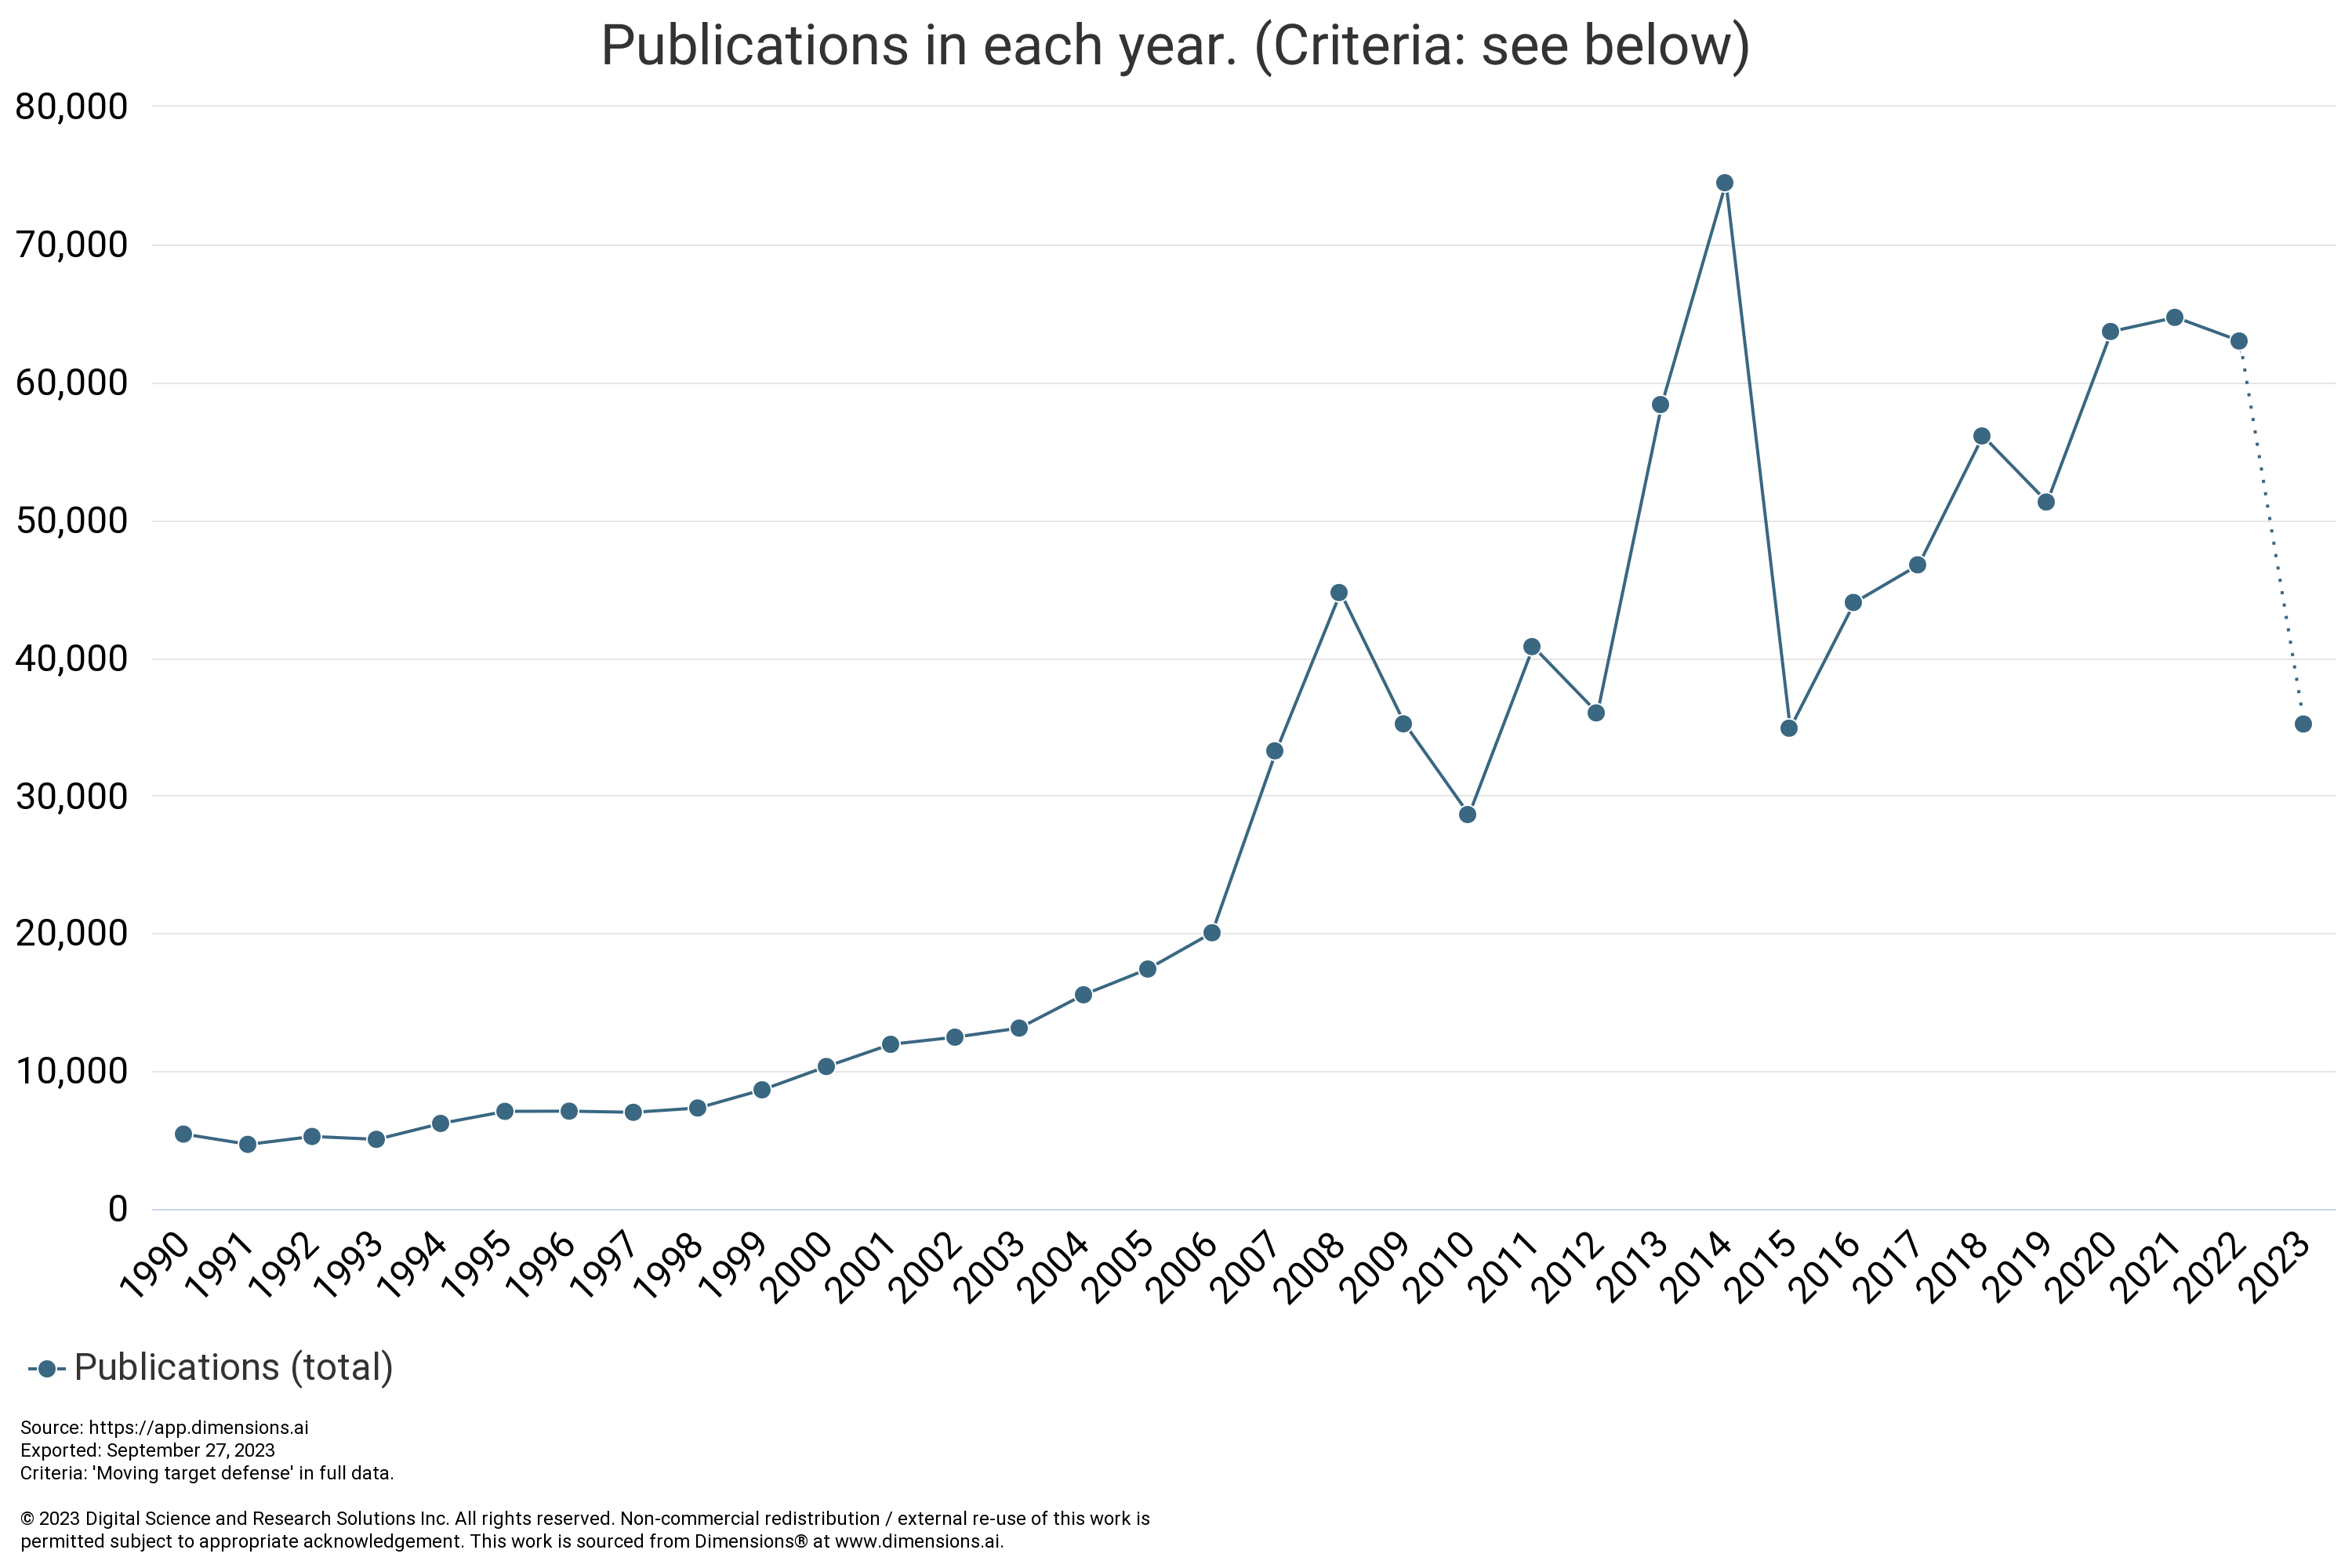
\includegraphics[width=\linewidth]{./imagenes/busquedasMTD.png}
    \caption{Investigaciones sobre MTD a lo largo del tiempo}
\end{figure}

A continuación vamos a hacer una revisión sobre los aspectos más importantes de los MTD, como son la clasificación y limitaciones. Además haremos un repaso sobre las implementaciones que se han realizado sobre servidores web, ya que es el objetivo de este trabajo.

\section{Clasificación}
Cuando queremos implementar un MTD, necesitamos elegir el componente más viable o donde necesitamos más protección.

\textbf{Qué mover}: debería ser un componente o atributo que habilite un vector de ataque. Por ejemplo, pueden ser una IP \cite{MTD-SDN+decoy}\cite{MTD-ipshuffling+honeypots}\cite{MTD-POC-empresa}, servidor web \cite{MTD-DARE}\cite{MTD-MORE+DARE+Java}, sistema operativo \cite{MTD-MORE+DARE+Java}, direcciones de memoria \cite{MTD-ASR}, base de datos \cite{MTD-arab}, WAF \cite{MTD-WAF}, VM \cite{MTD-POC-empresa}\cite{MTD-DARE}\cite{SCIT-base}, etc.

\textbf{Cómo moverlo}: una vez se ha seleccionado el componente, hay que determinar como cambiarlo, para esto hay tres opciones diferentes:
\begin{itemize}
    \item Mezcla: se cambia un componente por otro, los ejemplos de componentes incluyen direcciones IP de un servidor o las variables de entorno de un sistema.
    \item Diversidad: tiene componentes diferentes que realizan la misma tarea, por ejemplo, en vez de varios servidores Apache como servidores web, tiene un Apache y dos Nginx.
    \item Redundancia: tener componentes repetidos para asegurar que, si uno falla o es comprometido, otros pueden tomar su lugar o mitigar el impacto del ataque. 
\end{itemize}

\begin{figure}[h]
    \centering
    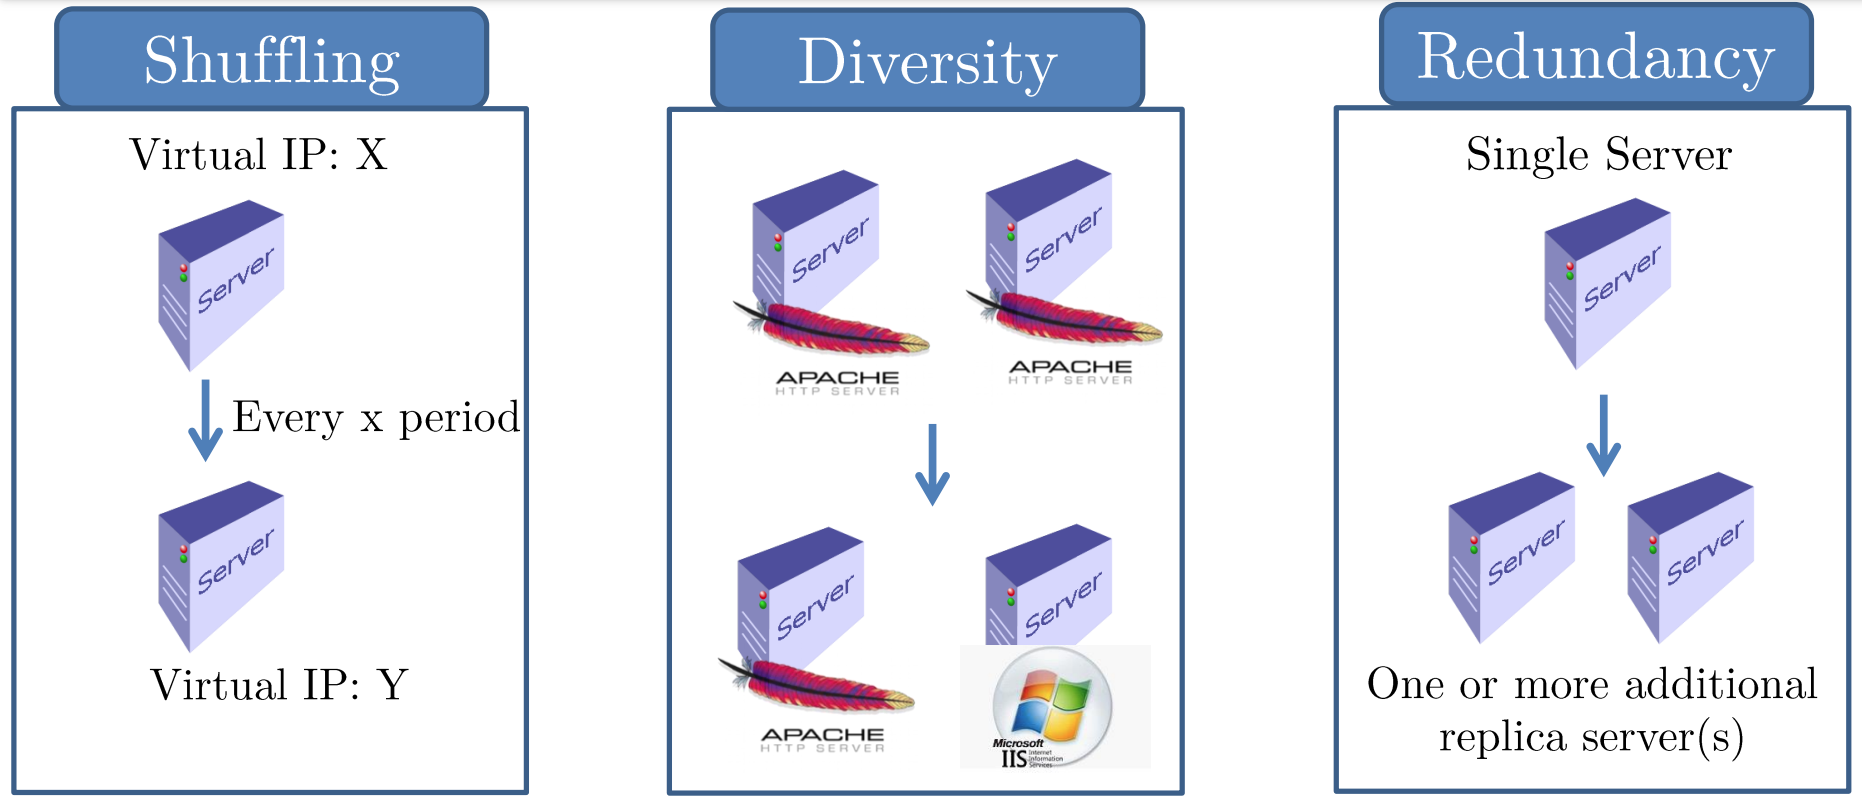
\includegraphics[width=\linewidth]{./imagenes/tiposmovimientos.png}
    \caption{Formas de mover un componente}
\end{figure}

\textbf{Cuándo moverlo}: una vez que se ha seleccionado el componente y la forma de moverlo, hay que determinar cuando moverlo. Hay dos opciones:
\begin{itemize}
    \item Por tiempo (proactivo): se mueve el componente de forma periódica, independientemente de si se ha detectado un ataque o no. El periodo no tiene por qué ser fijo, puede ser aleatorio o entre un rango de tiempo.
    \item Por evento (reactivo): se mueve el componente cuando se detecta un ataque o un fallo en el sistema, la forma de detectarlo puede ser machine learning\cite{MTD-ML}, uso de IPS\cite{Design-Generic-Intrusion-Tolerant-Architecture}, un WAF \cite{MTD-WAF}, etc.
\end{itemize}

Esta clasificación no es excluyente, es decir se pueden combinar diferentes opciones. Por ejemplo, se pueden combinar las dos opciones de cuando moverlo (creando una opción híbrida) con todas las opciones de como moverlo. La mayoría de veces una implementación combina varios de estas \cite{MTD-MORE+DARE+Java}\cite{MTD-DARE}\cite{MTD-arab}, aunque que exista esta posibilidad no quiere decir que se deban de mezclar todas las opciones posibles, ya que podrían dar configuraciones menos seguras o eficientes que al utilizar menos opciones \cite{MTD-comparativa-gorda}.

\section{Servidores web}
Los MTD basados en servidores web no es una de las principales líneas de investigación, ya que son más difíciles de adaptar a un entorno de producción, no hay consenso sobre ellos y no han demostrado tener resultados tan eficaces como otras líneas (SDN o \textit{IP shuffling}). Aun así, se han realizado varias implementaciones sobre estos, nos centraremos en aquellos que rotan los servidores que se utilizan, comenzando por el DARE (\textit{Dynamic Application Rotation Environment for Moving Target Defense}) este se basa en la estrategia utilizada por el MORE (\textit{Multiple Operating System Rotational Environment MTD})\cite{MORE}, la cual consiste en ir cambiando la máquina que recibe el tráfico mediante IP. DARE lo implementa en los puertos, esta consiste en rotar un servidor Nginx\cite{nginx} con uno Apache\cite{apache}, los cuales están en la misma máquina, para servir una página web estática. Esto lo logran utilizando un script como servicio el cual cambia la entrada de Iptables\cite{iptables} para apuntar a un puerto u otro.

El problema de DARE es que al actualizar el firewall, se perdía mucha disponibilidad al reiniciar el servicio, por lo que a partir de esta, surge \textit{DARE IMproved} (DIM). Este utiliza la misma estrategia que DARE, pero utiliza un script en Python el cual altera Iptables, pero no reinicia el servicio. Esto es posible, ya que si una regla está definida correctamente en Iptables, no es necesario reiniciarlo para que entre en funcionamiento, llevando la disponibilidad hasta el 98\%. Otra mejora que hace DIM respecto a DARE, es que redirige el tráfico a los servidores mediante el \textit{loopback}, lo que permite que los servidores no sean accesibles desde fuera de la máquina. Con estas mejoras se consiguieron aumentar la disponibilidad, rendimiento y la seguridad.

A pesar de las mejoras llevadas a cabo, la disponibilidad sigue sin ser suficiente, algunos sitios web deben tener una disponibilidad del 99.99\% para cumplir con el acuerdo de nivel de servicio (SLA)\cite{SLA}, al modificar Iptables, los paquetes que estaban siendo procesados por el servidor son descartados automáticamente. Por lo que surge \textit{Mutable Asymmetric web Server Security} (MASS), el cual está basado en las implementaciones anteriores, con las siguientes mejoras:
\begin{itemize}
    \item Utiliza Firewalld\cite{firewalld}: es una alternativa a Iptables, la cual tampoco reinicia el servicio. Además, este puede controlar el flujo de paquetes, por lo que mientras que un servidor está siendo cambiado, los paquetes son almacenados en una cola para ser enviados al acabar el cambio.
    \item Uso de contenedores: ahora cada servidor está en un contenedor diferente, lo que aumenta el aislamiento, ya que si anteriormente si un servidor era comprometido, toda la máquina lo era también.
    \item Reencarnación de contenedores: esta técnica consiste en que una vez que un contenedor es cambiado por el otro contenedor, en vez de mantenerlo o comprobar si ha sido comprometido, es destruido directamente, para volver a crear un contenedor nuevo a partir de una imagen base.
\end{itemize}

Alejándose de la línea anterior, otra implementación es la de Philip Tibom y Max Buck\cite{MTD-gotemburgo}, en la que utilizan nodos de Kubernetes\cite{kubernetes} para implementar el MTD. Esta configuración consigue un 100\% de disponibilidad. Utiliza \textit{VM shufflig}, cambiando los nodos entre diferentes ubicaciones físicas y su IP. Está preparado para utilizar distintas imágenes de Docker en diferentes nodos.

El SCIT (\textit{Self Cleansing Intrusion Tolerance})\cite{SCIT-base} es otra tecnología vinculada a los servidores web. Esta estrategia se basa en la reencarnación de un componente, similar a lo que realiza MASS. En 2011, se publicó un estudio\cite{SCIT-cloud}, que compartía estructura con el trabajo de Philip Tibom y Max Buck; sin embargo, en este caso se implementaba el SCIT. Es notable mencionar que, pese a los 11 años transcurridos desde ambas investigaciones, no se ha liberado ningún software de código abierto que emulase dicha implementación.

% investigar a fondo ancor y ver si tiene lugar aqui

\section{Limitaciones}
A pesar de las diferentes investigaciones e implementaciones que existen, muchas tienen en común algunas malas prácticas y clichés que se repiten, dando lugar a un análisis erróneo de los resultados. Estas prácticas son:
\begin{itemize}
    \item Pruebas de explotación pobres: la evaluación de la defensa se suele centrar en la fase de reconocimiento, para después utilizar un único \textit{exploit} en la explotación por componente, esto hace las pruebas más fáciles, pero no da una visión realista de la seguridad, ya que utiliza un único vector de ataque, el cual no varía el tiempo que se tarda en explotar la vulnerabilidad.
    \item MTD por eventos o híbridos dejados atrás: las investigaciones e implementaciones se suelen centrar en MTD proactivos, ya que una de las características que se le atribuye a los MTD es que son inseguros por defecto. Por lo que las líneas principales de investigación se centran en mantener el rendimiento, ofuscar el reconocimiento y reducir el tiempo que un componente es vulnerable. Si bien es cierto que los MTD proactivos pueden cumplir con estos objetivos y la mayor parte de la investigación debería seguir esa línea, dejar de lado los eventos se aleja de una solución realista, por un ejemplo tan sencillo como que en un MTD con diversidad o redundancia de servidores, uno de ellos esté caído y se le siga mandando tráfico.
    \item Aumento de la superficie de ataque: en determinados MTD proactivos la rotación de un componente puede aumentar las brechas de seguridad\cite{MTD-critica}, este es un problema intrínseco a esta tecnología, que se suele pasar por alto en la mayoría de investigaciones. Se podrían dar las siguientes situaciones como ejemplo:
    \begin{enumerate}
        \item Tenemos un componente seguro y otro inseguro: si rotamos entre ellos cada cierto tiempo, el sistema será vulnerable la mitad del tiempo. La solución realista sería dejar de cambiar al vulnerable al detectar el ataque.
        \item Si tenemos dos componentes seguros: el sistema no será vulnerable nunca, si los componentes son diferentes uno rendirá mejor que el otro. La solución realista sería mantener el componente que mejor rendimiento tenga, y si los componentes son iguales, no haría falta rotarlos, una configuración estática sería más óptima.
        \item Tenemos dos componentes inseguros: el sistema será vulnerable siempre. La solución realista sería realizar cambios constantemente hasta parchear las vulnerabilidades, que serían dos en vez de una.
    \end{enumerate}
    Como hemos dicho antes estos ejemplos no aplican a todas las tecnologías MTD, pero son uno de los problemas de raíz de esta tecnología.
    \item Atribuir la seguridad al cambio erróneamente: es decir realizamos una rotación entre diferentes componentes, pero el cambio no es gracias a utilizar un componente diferente. Un ejemplo, tenemos una vulnerabilidad que causa una denegación de servicio (DOS) en un servidor, esta tarda 30 s en empezar a funcionar y 60 s en dejar el servidor caído. Si realizamos cambios cada 15 s entre el servidor vulnerable y uno seguro (reiniciando el servidor al cambiarlo), el servidor nunca estará caído, pero no es gracias a la rotación, sino al reinicio. Si realizáramos la rotación entre dos servidores vulnerables, el servidor tampoco estaría caído, ya que el tiempo de explotación es mayor que el del cambio de componente.
    \item Falta de código \textit{opensource}: apenas hay código abierto sobre los MTD, esto hace que sea difícil replicar los resultados de las investigaciones, ya que no se puede saber si se ha implementado correctamente o no. Además de retrasar la investigación al tener que reinventar la rueda y no poder realizar comparativas entre soluciones.
\end{itemize}

\section{Analogías}

Alexander Bajic y Georg T. Becker listaron una serie de analogías\cite{MTD-critica} con los ejemplos anteriores:
\begin{itemize}
    \item El combate aéreo y bandada de pájaros: en un combate aéreo, un piloto debe hacer maniobras impredecibles para no ser un blanco fácil. Esta situación ilustra cómo las tácticas de seguridad de TI actuales son estáticas, como esperar en un búnker. Algunas empresas usan la analogía de una bandada de pájaros, donde cada ave se mueve constantemente, dificultando que un depredador ataque a una específica.
    \item La caza del ciervo: Un ciervo en movimiento puede eludir a un cazador que lo persigue. Sin embargo, si el cazador espera en un punto, dicho movimiento es lo que lo pone en peligro. Es vital considerar no solo cómo este beneficia a la defensa, sino también cómo podría beneficiar al atacante. Un ejemplo de esto es el aumento de superficie de ataque que se mencionó anteriormente.
    \item El trilero: una bola se esconde bajo uno de los tres cubiletes que se mueven rápidamente. Sin embargo, este juego suele ser un engaño, ya que el operador manipula sigilosamente la bola. Aunque el movimiento de los cubiletes puede no ser el factor de seguridad en la MTD, otros aspectos de la defensa sí lo son.
\end{itemize}

\begin{figure}[h]
    \centering
    \begin{minipage}{.3\textwidth}
        \centering
        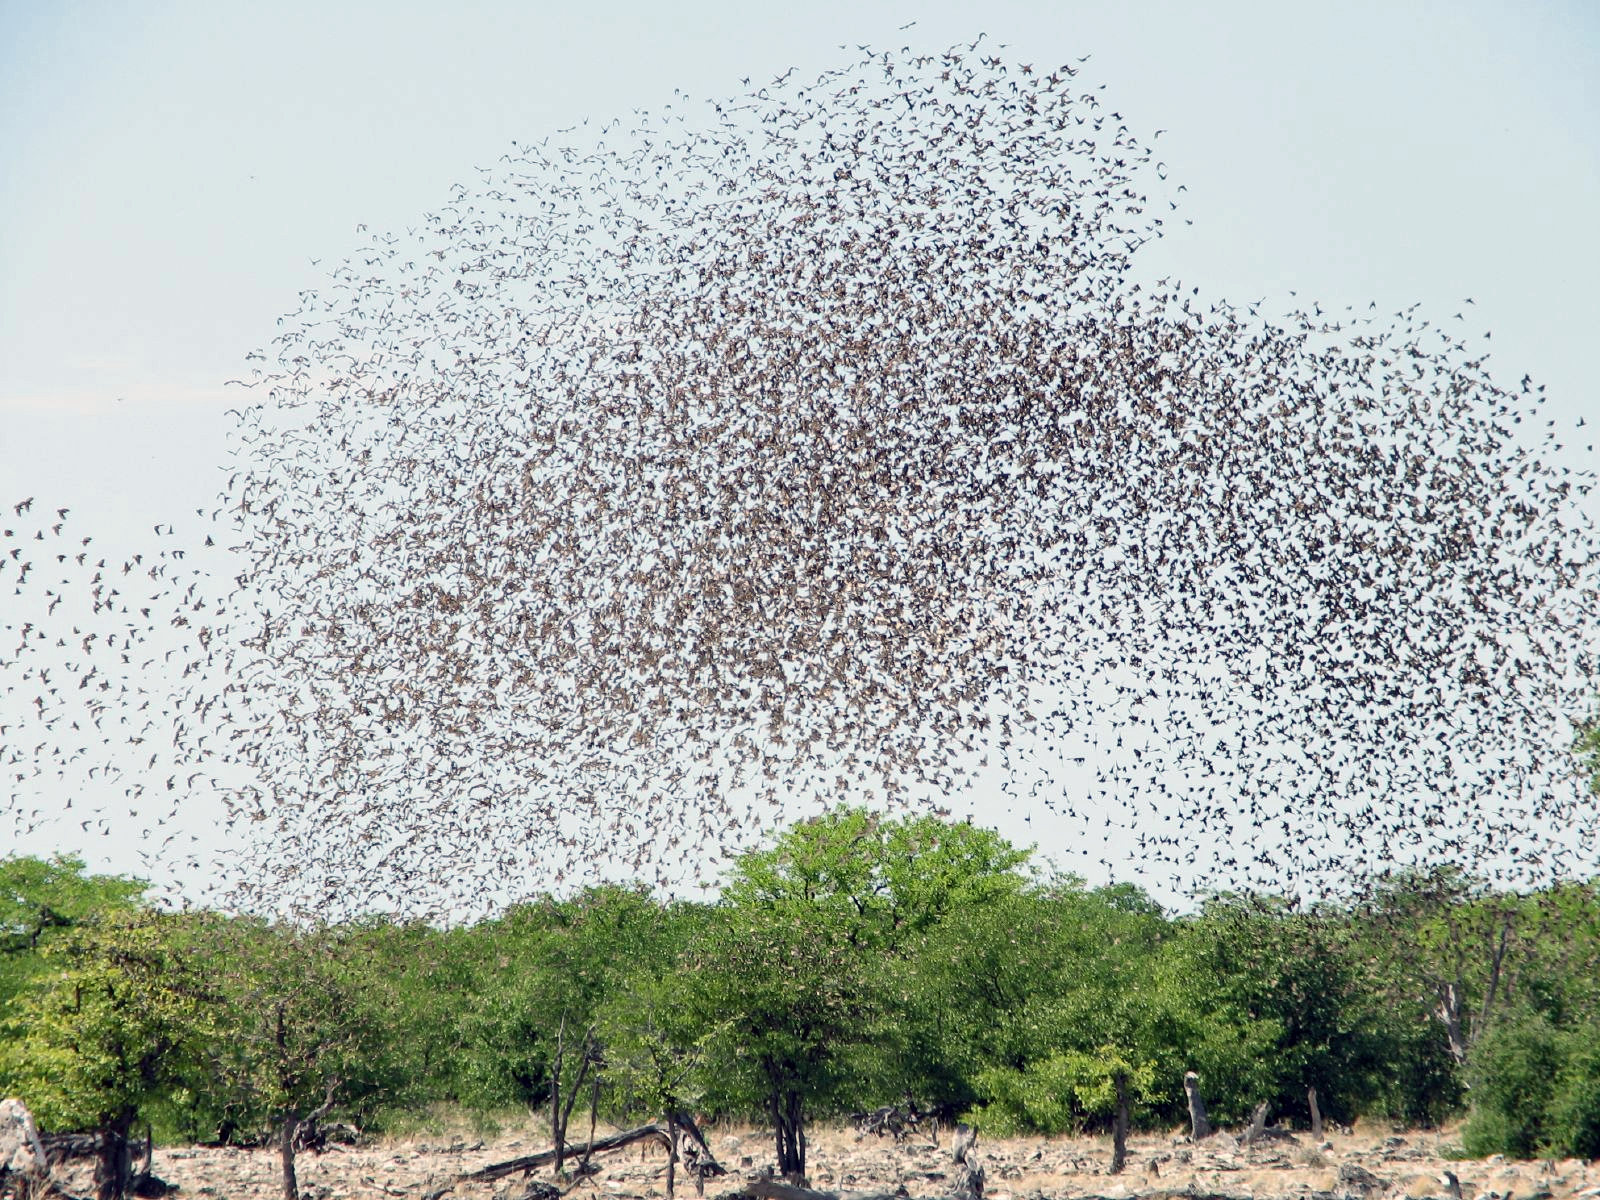
\includegraphics[width=\linewidth]{./imagenes/bandada.jpg}
        \caption{Bandada de pájaros}
    \end{minipage}
    \hfill
    \begin{minipage}{.3\textwidth}
        \centering
        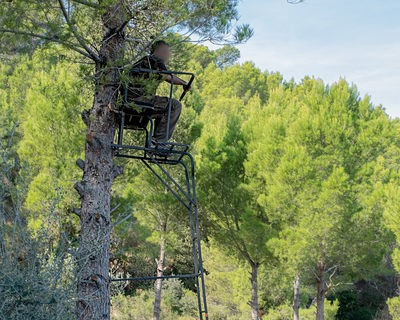
\includegraphics[width=\linewidth]{./imagenes/caza.jpg}
        \caption{Cazador esperando que el ciervo se ponga a tiro}
    \end{minipage}
    \hfill
    \begin{minipage}{.3\textwidth}
        \centering
        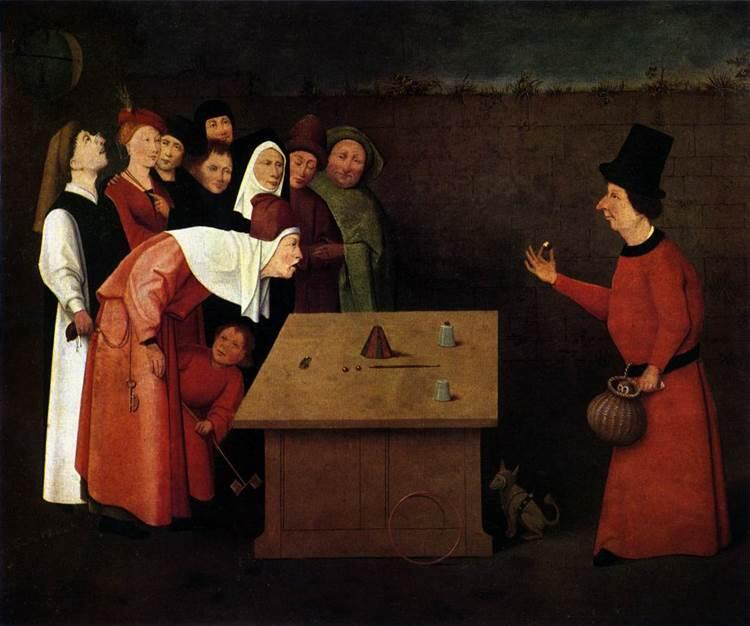
\includegraphics[width=\linewidth]{./imagenes/trilero.jpg}
        \caption{Trilero}
    \end{minipage}
\end{figure}



% cuarta pregunta impacto del movimiento

% y a día de hoy no existe un software que la implemente totalmente(((Dejar así hasta que compruebe ANCOR en Openstack))). Esto se debe a que es una tecnología que no esta madurada, es decir, sigue siendo un tema de debate a día de hoy, ya que no se sabe con exactitud en que casos es útil o rentable utilizarla, y por otro lado al no haber herramientas de código abierto con esta técnica, no se conoce su viabilidad en entornos de producción.

	
	\chapter{Planificación}

\section{Metodología utilizada}
La realización de este proyecto se ha llevado a cabo con \textbf{desarrollo ágil}, según Deisy Villalba: ``El desarrollo ágil de software es una forma de integrar las capacidades de un equipo de desarrollo para poner en marcha un plan de trabajo que permita ir entregando pequeños resultados al cliente en poco tiempo, para que este se sienta tranquilo y a gusto con el trabajo realizado. Además, se prima el flujo de trabajo, la colaboración entre los miembros del equipo y siempre enfocarse en lo que se está haciendo y cómo se está haciendo.''\cite{desarrollo-agil}.

O de una forma más sencilla, esta metodología nos dice:
\begin{enumerate}
    \item ¿Qué tengo que hacer ahora?
    \item ¿Es correcta la solución que he planteado al problema que estoy resolviendo?
\end{enumerate}

\section{Temporización}

\section{Seguimiento del desarrollo}

Se han llevado a cabo los siguientes hitos:
\begin{enumerate}
    \item Preparar el entorno para la documentación.
    \item Redactar la introducción.
    \item Redactar el estado del arte.
    % \item Implementación del \textit{MASS}.
\end{enumerate}

	% % Análisis del problema
	% % 1. Análisis de requisitos
	% % 2. Análisis de las soluciones
	% % 3. Solucion propuesta
	% % 4. Análisis de seguridad
	% \input{secciones/05_analisis}

	% Desarrollo bajo sprints: 
	% 	1. Permitir registros y login de usuarios
	% 	2. Desarrollo del sistema de incidencias
	% 	3. Desarrollo del sistema de denuncias administrativas y accidentes
	% 	4. Desarrollo del sistema de croquis
	%   5. Instalación de la aplicación de manera automática
	% \chapter{Implementación}

La implementación del software se ha dividido en hitos. Estos han sido definidos en Github
y cada uno de ellos contiene un grupo de \textit{issues} que se corresponden con las distintas
mejoras que se han ido incorporando al software a lo largo de su desarrollo.

\section{Toma de decisiones}

\subsection{Gestor de dependencias}
Los criterios para elegir el gestor de dependencias, de mayor a menor prioridad, han sido:
\begin{enumerate}
    \item Soporte pyproject.toml.
    \item Creación de entornos virtuales/gestión las dependencias de forma local.
    \item Rendimiento.
\end{enumerate}

Donde se van a evaluar los siguientes gestores de dependencias: \textit{Pipenv, Poetry, Hatch, PDM, Conda, Mamba, Pixi, Rye, Miniconda y Micromamba}

\begin{table}[H]
    \centering
    \begin{adjustbox}{width=\textwidth, totalheight=\textheight, keepaspectratio}
        \begin{tabular}{|c|c|c|c|c|c|c|c|c|c|c|c|c|}
            \hline
            Requisitos & Pipenv & Poetry & Hatch & PDM & Conda & Mamba & Pixi & Rye & Pip & Pip-tools & Miniconda & Micromamba\\
            \hline
            Pyproject.toml & \checkmark & \checkmark & \checkmark & \checkmark & \ding{55} & \ding{55} & \ding{55} & \checkmark & \ding{55} & \ding{55} & \ding{55} & \ding{55} \\
            Entornos virtuales & \checkmark & \checkmark & \checkmark & \checkmark & \checkmark & \checkmark & \checkmark & \checkmark & \ding{55} & \ding{55}  & \checkmark & \checkmark \\
            \hline
        \end{tabular}
    \end{adjustbox}
    \caption{Comparativa entre gestores de dependencias.}
\end{table}

Pip y pip-tools, no gestionan entornos virtuales, el resto de opciones si lo hace. Conda, mamba y sus versiones lite no tienen pyprojec.toml, en cuanto a pixi, este está basado sobre conda, pero genera en el directorio de trabajo su pixi.lock y pixi.toml, el cual no cumple con el estándar de pyproject.toml.

Para evaluar su rendimiento nos basaremos en diferentes benchmarks\cite{pm-benchmark-shootout}. Donde observamos que poetry es el más rápido en realizar la instalación desde un lockfile, creación de este y en añadir un paquete. Además es el segundo en actualizar los paquetes. Sin embargo es el que más tarda en ser instalado. Ya que el gestor de dependencias será instalado una sola vez, vamos a priorizar los otros benchmarks. Por lo que tenemos a poetry como ganador ante PDM y pipenv.

Debido a que no se ha encontrado ningún benchmark sobre Hatch y Rye (este además de que está en un estado experimental), se utilizará poetry como gestor de dependencias.

\subsection{Gestor de tareas}
Los criterios para elegir el gestor de tareas, de mayor a menor prioridad, han sido:
\begin{enumerate}
    \item Curva de aprendizaje.
    \item Ficheros de configuración.
\end{enumerate}

Donde se van a evaluar los siguientes gestores de tareas: \textit{Poethepoet, Pypyr, Invoke, Doit, Pytask}

\begin{table}[H]
    \centering
    \begin{adjustbox}{width=\textwidth, totalheight=\textheight, keepaspectratio}
        \begin{tabular}{|c|c|c|c|c|c|}
        \hline
        Requisitos & Poethepoet & Pypyr & Invoke & Doit & Pytask\\
        \hline
        Curva de aprendizaje & Fácil & Difícil & Medio & Medio & Medio \\
        Ficheros de configuración & pyproject.toml & pipelines/*.yml + .py & tasks.py & dodo.py & task\_*.py \\
        \hline
        \end{tabular}
    \end{adjustbox}
      \caption{Comparativa entre gestores de tareas.}
\end{table}

De las opciones anteriores, poethepoet es el que menos deuda técnica aporta al proyecto, ya que además de permitir funciones en Python como invoke, doit y pytask, permite utilizar shell, comandos y expresiones en Python directamente. Sumando que utiliza el fichero de configuración pyproject.toml, por lo que se evitarían ficheros extra.


\subsection{Test runner}
Los criterios para elegir el \textit{test runner}, de mayor a menor prioridad, han sido:
\begin{enumerate}
    \item BDD (Gherkin).
    \item Estructura de archivos.
    \item Diferentes características.
\end{enumerate}

Donde se van a evaluar las siguientes herramientas: \textit{Pytest, Nose2, Unittest, Green, Behave, Testcontainers, Doctest, Radish}

\begin{table}[H]
    \centering
    \begin{adjustbox}{width=\textwidth, totalheight=\textheight, keepaspectratio}
        \begin{tabular}{|c|c|c|c|c|c|c|c|c|}
        \hline
        Requisitos & Pytest & Nose2 & Unittest & Green & Behave & Testcontainers & Doctest & Radish \\
        \hline
        BDD & \checkmark (plugin) & \ding{55} & \ding{55} & \ding{55} & \checkmark & \ding{55} & \ding{55} & \checkmark \\
        \hline
        \end{tabular}
    \end{adjustbox}
      \caption{1ª Comparativa entre gestores de tareas.}
\end{table}

Se descartan todas excepto Pytest, Behave y Radish.

La estructura de archivos entre estos apenas varía, todos utilizan \textit{steps}, \textit{features} y un fichero \textit{.ini} (el cual puede ser utilizado para cambiar la estructura).

En este punto los tres son válidos en el proyecto, sin embargo, vamos a comparar algunas características para seleccionar uno:

\begin{itemize}
    \item Paralelismo: Behave no tiene paralelismo nativo (y el plugin que lo soportaba esta deprecated), mientras que Radish lo soporta de forma nativa y Pytest con un plugin (pytest-xdist).
    \item Escenario como precondición: Radish permite que para ejecutarse un escenario se tenga que cumplir otro previamente.
    \item Bucle de escenario: Radish permite ejecutar escenarios en bucle.
    \item Declaración explícita de escenarios: Pytest necesita que en el fichero \textit{steps} se declare explícitamente el escenario.
    \begin{table}[H]
        \centering
        \begin{adjustbox}{width=\textwidth, totalheight=\textheight, keepaspectratio}
            \begin{tabular}{|c|c|c|c|}
            \hline
            Otras características & Pytest & Behave & Radish \\
            \hline
            Dependencias & 11 & 4 & 9 \\
            \hline
            Tamaño & 1.25 MB & 840 KB & 1.89 MB \\
            \hline
            Forks (Github) & 206 & 679 & 48 \\
            \hline
            Stars (Github) & 1.2 K & 3 K & 176 \\
            \hline
            \end{tabular}
        \end{adjustbox}
            \caption{2ª Comparativa entre gestores de tareas.}
    \end{table}
\end{itemize}


En esta comparativa se puede ver que Pytest se queda un poco atrás en la facilidad de uso de BDD, mientras que Radish es el que tiene más funcionalidades. Sin embargo estas funcionalidades, como el paralelismo, no se aplicarán a este proyecto, ya que los test modificarán iptables de la máquina donde se ejecute y levantará contenedores, aunque estas tareas podrían ser paralelizables, debido a su complejidad no se realizarán. Otra funcionalidad como los bucles de escenarios no será necesario y los escenarios como precondición podrían ser útiles en otro contexto, ya que este se podría utilizar para comprobar que el docker está corriendo correctamente, pero esto se adaptaría mejor en el \textit{setup} y \textit{teardown} (utilizando menos recursos), por lo que, aunque Radish brinda más funcionalidades, difícilmente serán adaptables a este proyecto, por lo que se va a utilizar Behave el cual cumple con los requisitos necesarios, es el que añade menos dependencias, es el más ligero y cuenta con mayor comunidad (dentro de BDD).


\subsection{Librería de aserciones}
Los criterios para elegir la librería de aserciones, de mayor a menor prioridad, han sido:

\begin{enumerate}
    \item Por defecto.
    \item Otras características.
\end{enumerate}

Donde se van a evaluar las siguientes librerías: \textit{Assert, Unittest, PyHamcrest, Pytest, Asserpy, Truth, Matchers, Grappa, Verify}

Se descartarán todos excepto Assert y Unittest, los cuales están incluidos por defecto en Python.

Se utilizará Unittest, ya que aunque no se necesite gran variedad de funcionalidades y se pueda conseguir lo mismo con ambas, Unittest permitirá no tener que escribir explícitamente los fallos (lo cual sería más necesario si no se utilizase un BDD) y usar una función autodescriptiva, consiguiendo una mayor legibilidad.

	% % Presupuesto

	% % Conclusiones
	% \input{secciones/07_conclusiones}

	% Trabajos futuros


	
	\newpage
	\bibliography{bibliografia}
	\bibliographystyle{plain}
	
\end{document}

